\chapter{METODOLOGI}
\label{chap:metodologi}
\section{Block Diagram Metodologi}
Penelitian ini dilaksanakan sesuai dengan desain sistem seperi Gambar \ref{fig:block}. Desain sistem merupakan konsep dari
pembuatan dan perancangan infrastruktur dan kemudian diwujudkan dalam bentuk blok-blok alur yang harus dikerjakan. Gambar \ref{fig:block} menunjukkan bagan umum metodologi sistem.
\setlength{\belowcaptionskip}{-5pt}
\begin{center}
	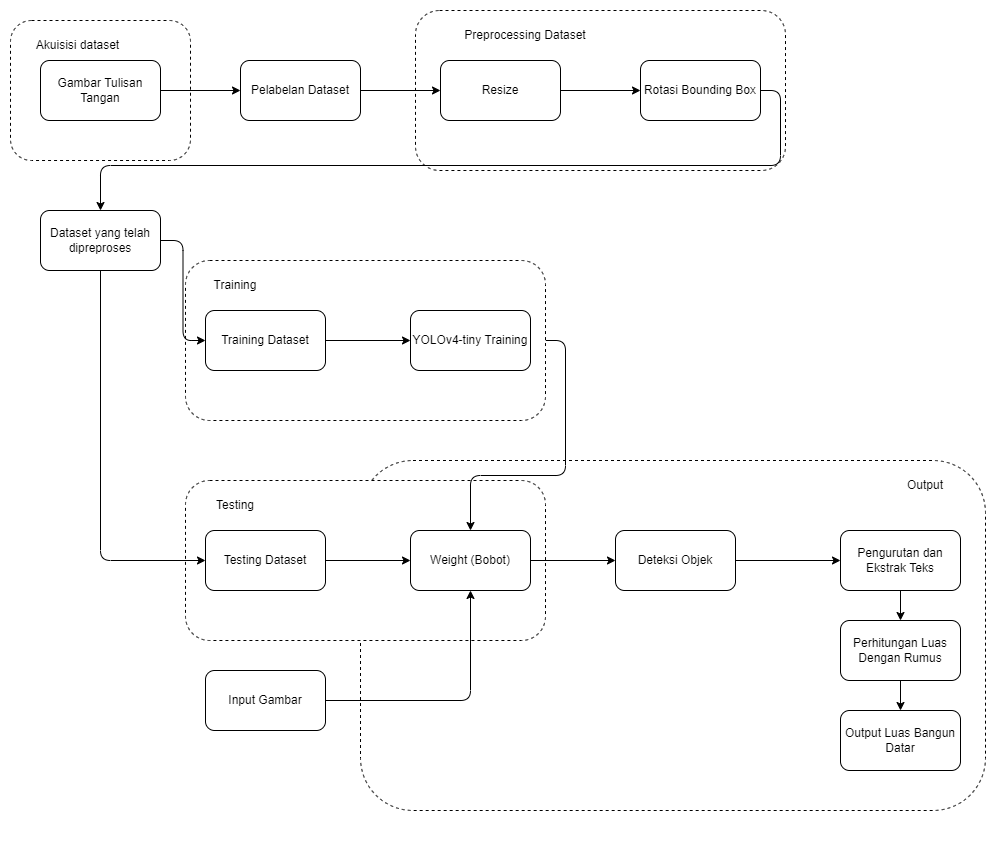
\includegraphics[width=0.85\textwidth]{gambar/block diagram baru.png}
	\captionof{figure}{Block Diagram Metodologi}
	\label{fig:block}
\end{center}

\subsection{Dataset}
\label{subsection:Dataset}
Proses pengumpulan dataset gambar bangun datar dan parameter pada papan tulis dilakukan dengan menuliskan sejumlah huruf parameter bangun datar dan gambar bangun datar pada media papan tulis kemudian dilakukan proses pengambilan foto. Proses tersebut diulang selama beberapa kali untuk setiap kelas parameter bangun datar dan gambar bangun datar. Seluruh tulisan parameter dan gambar bangun datar pada papan tulis ditulis oleh 1 orang yang sama, jumlah dataset seluruhnya adalah 269 gambar. Gambar \ref{fig:persegiDataset} sampai Gambar \ref{fig:trapesiumDataset} merupakan foto dataset citra gambar dan parameternya pada papan tulis.
\begin{center}
	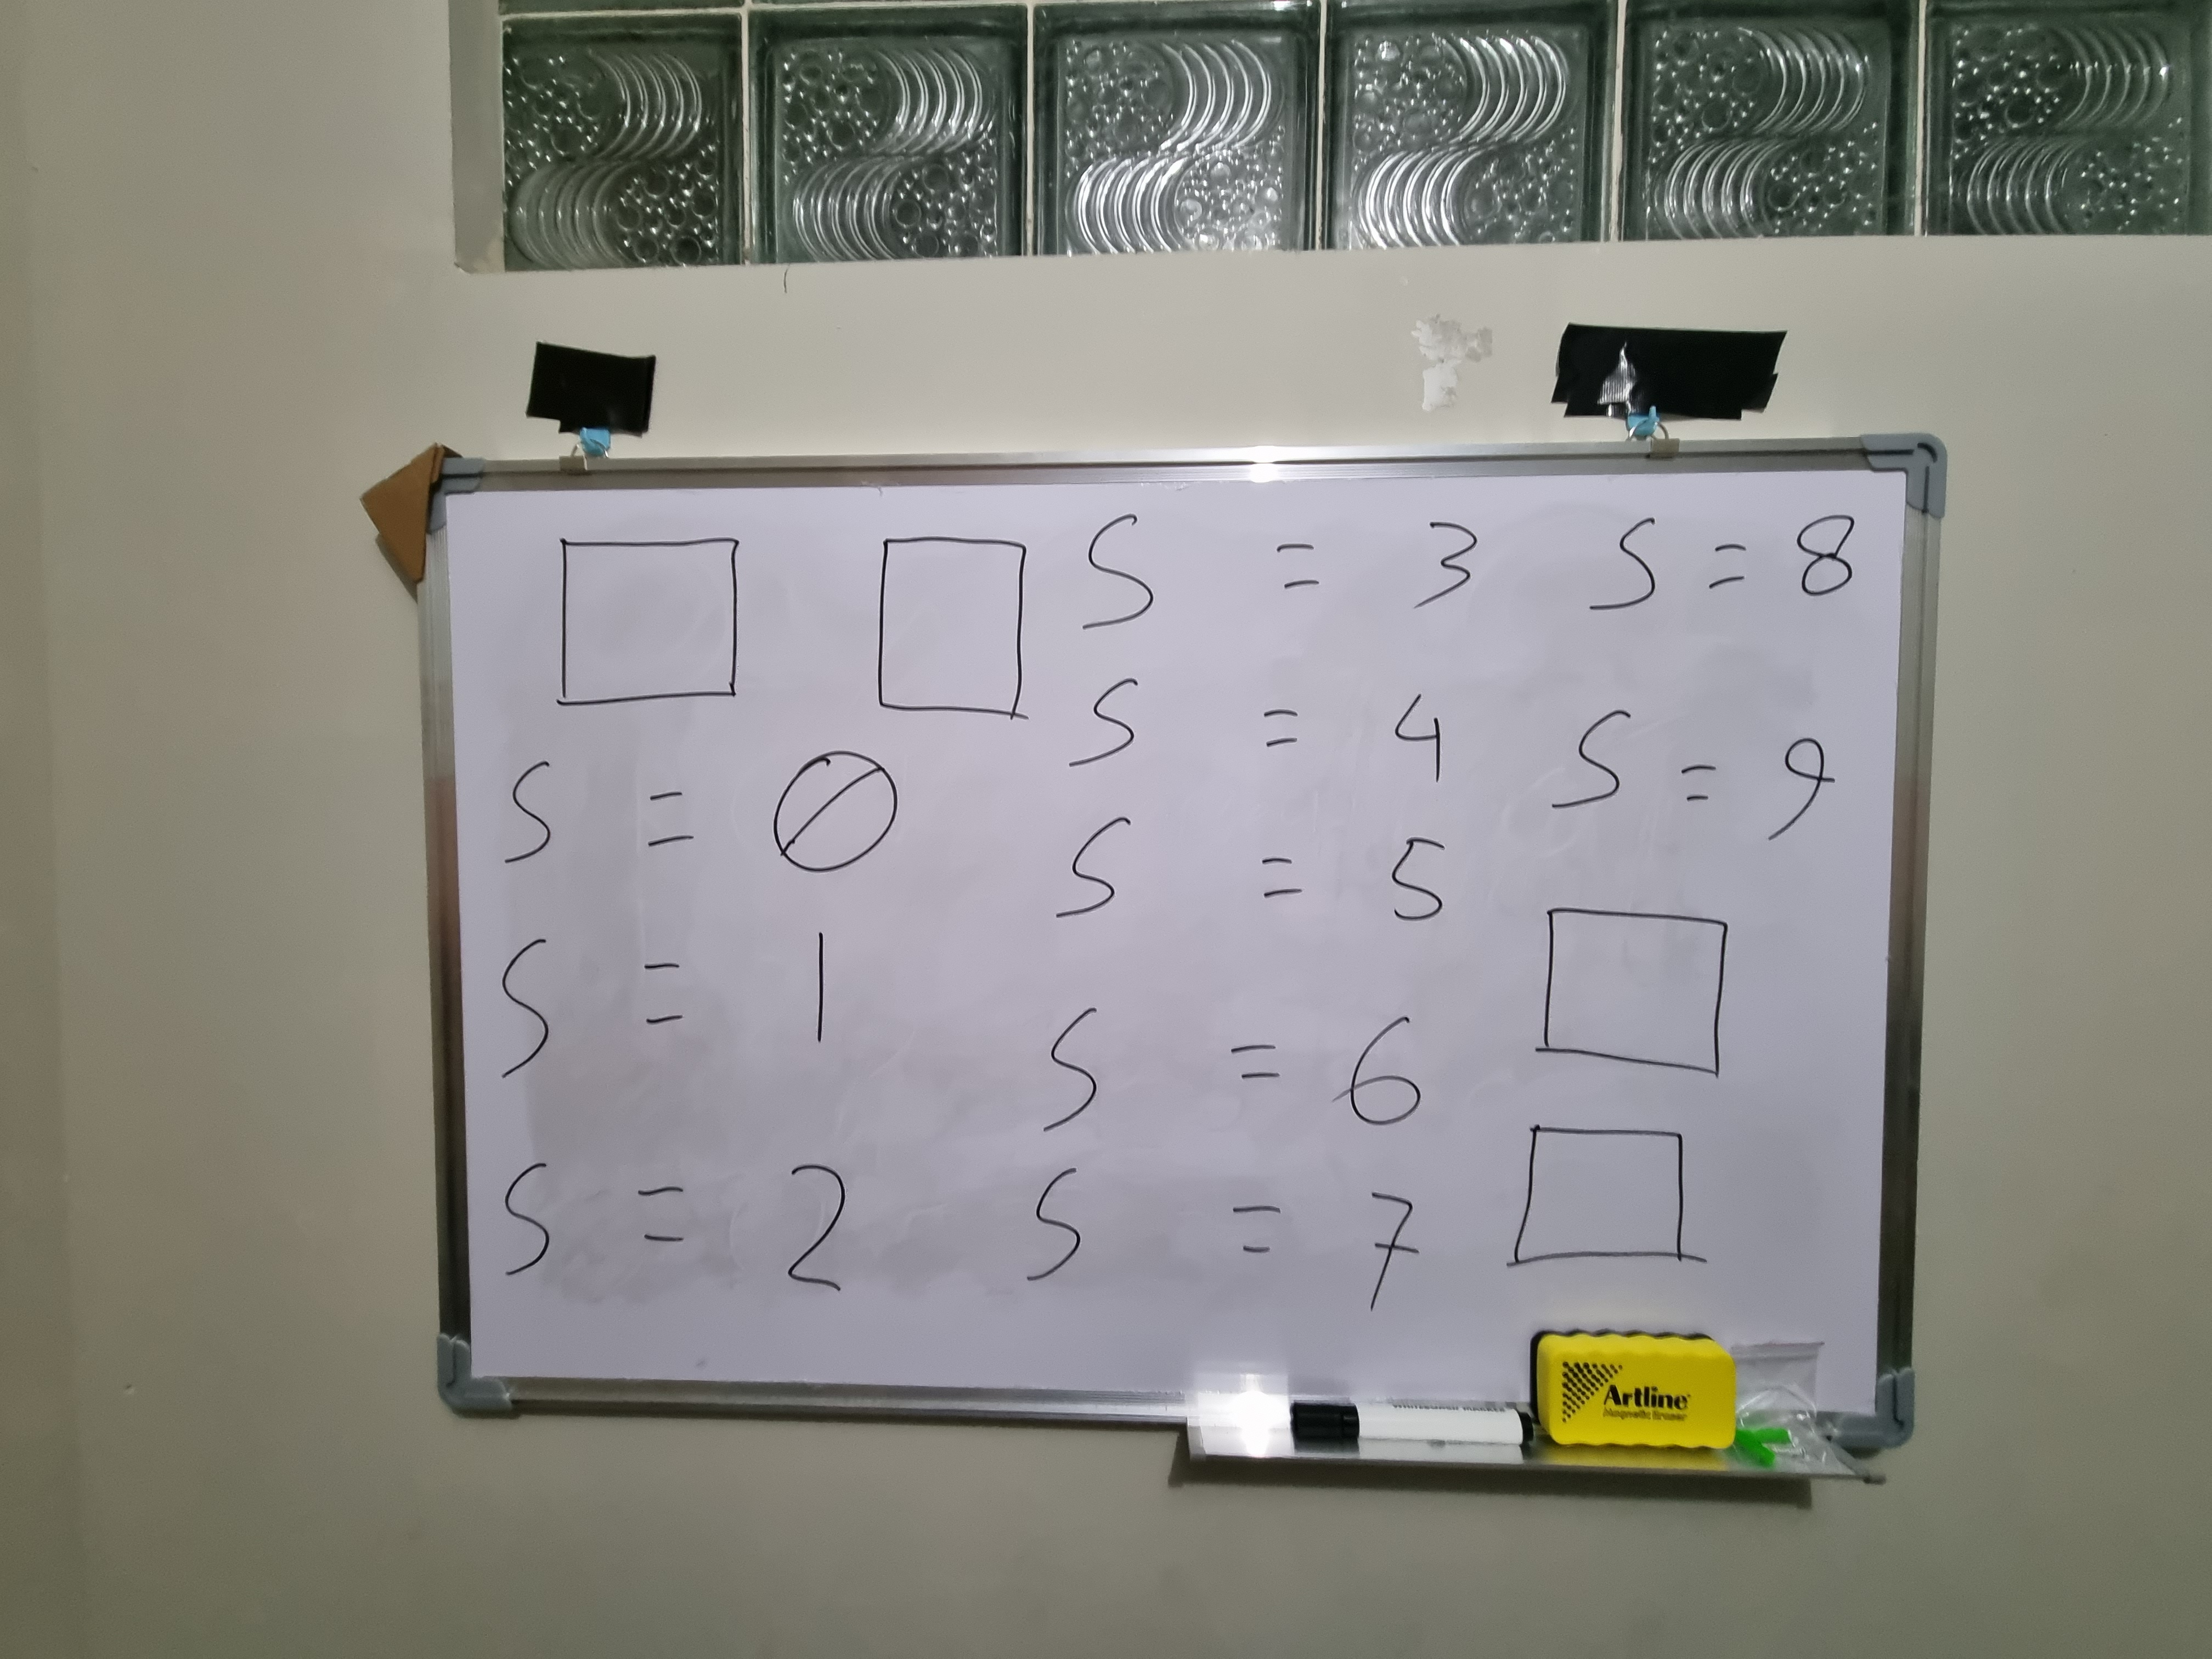
\includegraphics[width=0.55\textwidth]{gambar/BangunParameter.jpg}	
	\captionof{figure}{Contoh Citra Gambar dan Parameter Bangun Persegi}
	\label{fig:persegiDataset}
\end{center}
Pada Gambar \ref{fig:persegiDataset} didapatkan gambar bangun datar persegi yang merupakan objek bangun datar yang akan dideteksi oleh program. Selain itu huruf "S" merupakan parameter yang akan dideteksi oleh program untuk mengetahui paramter dari sebuah bangun datar persegi. Angka "0" sampai "9" merupakan objek angka yang digunakan untuk perhitungan luas persegi.

\begin{center}
	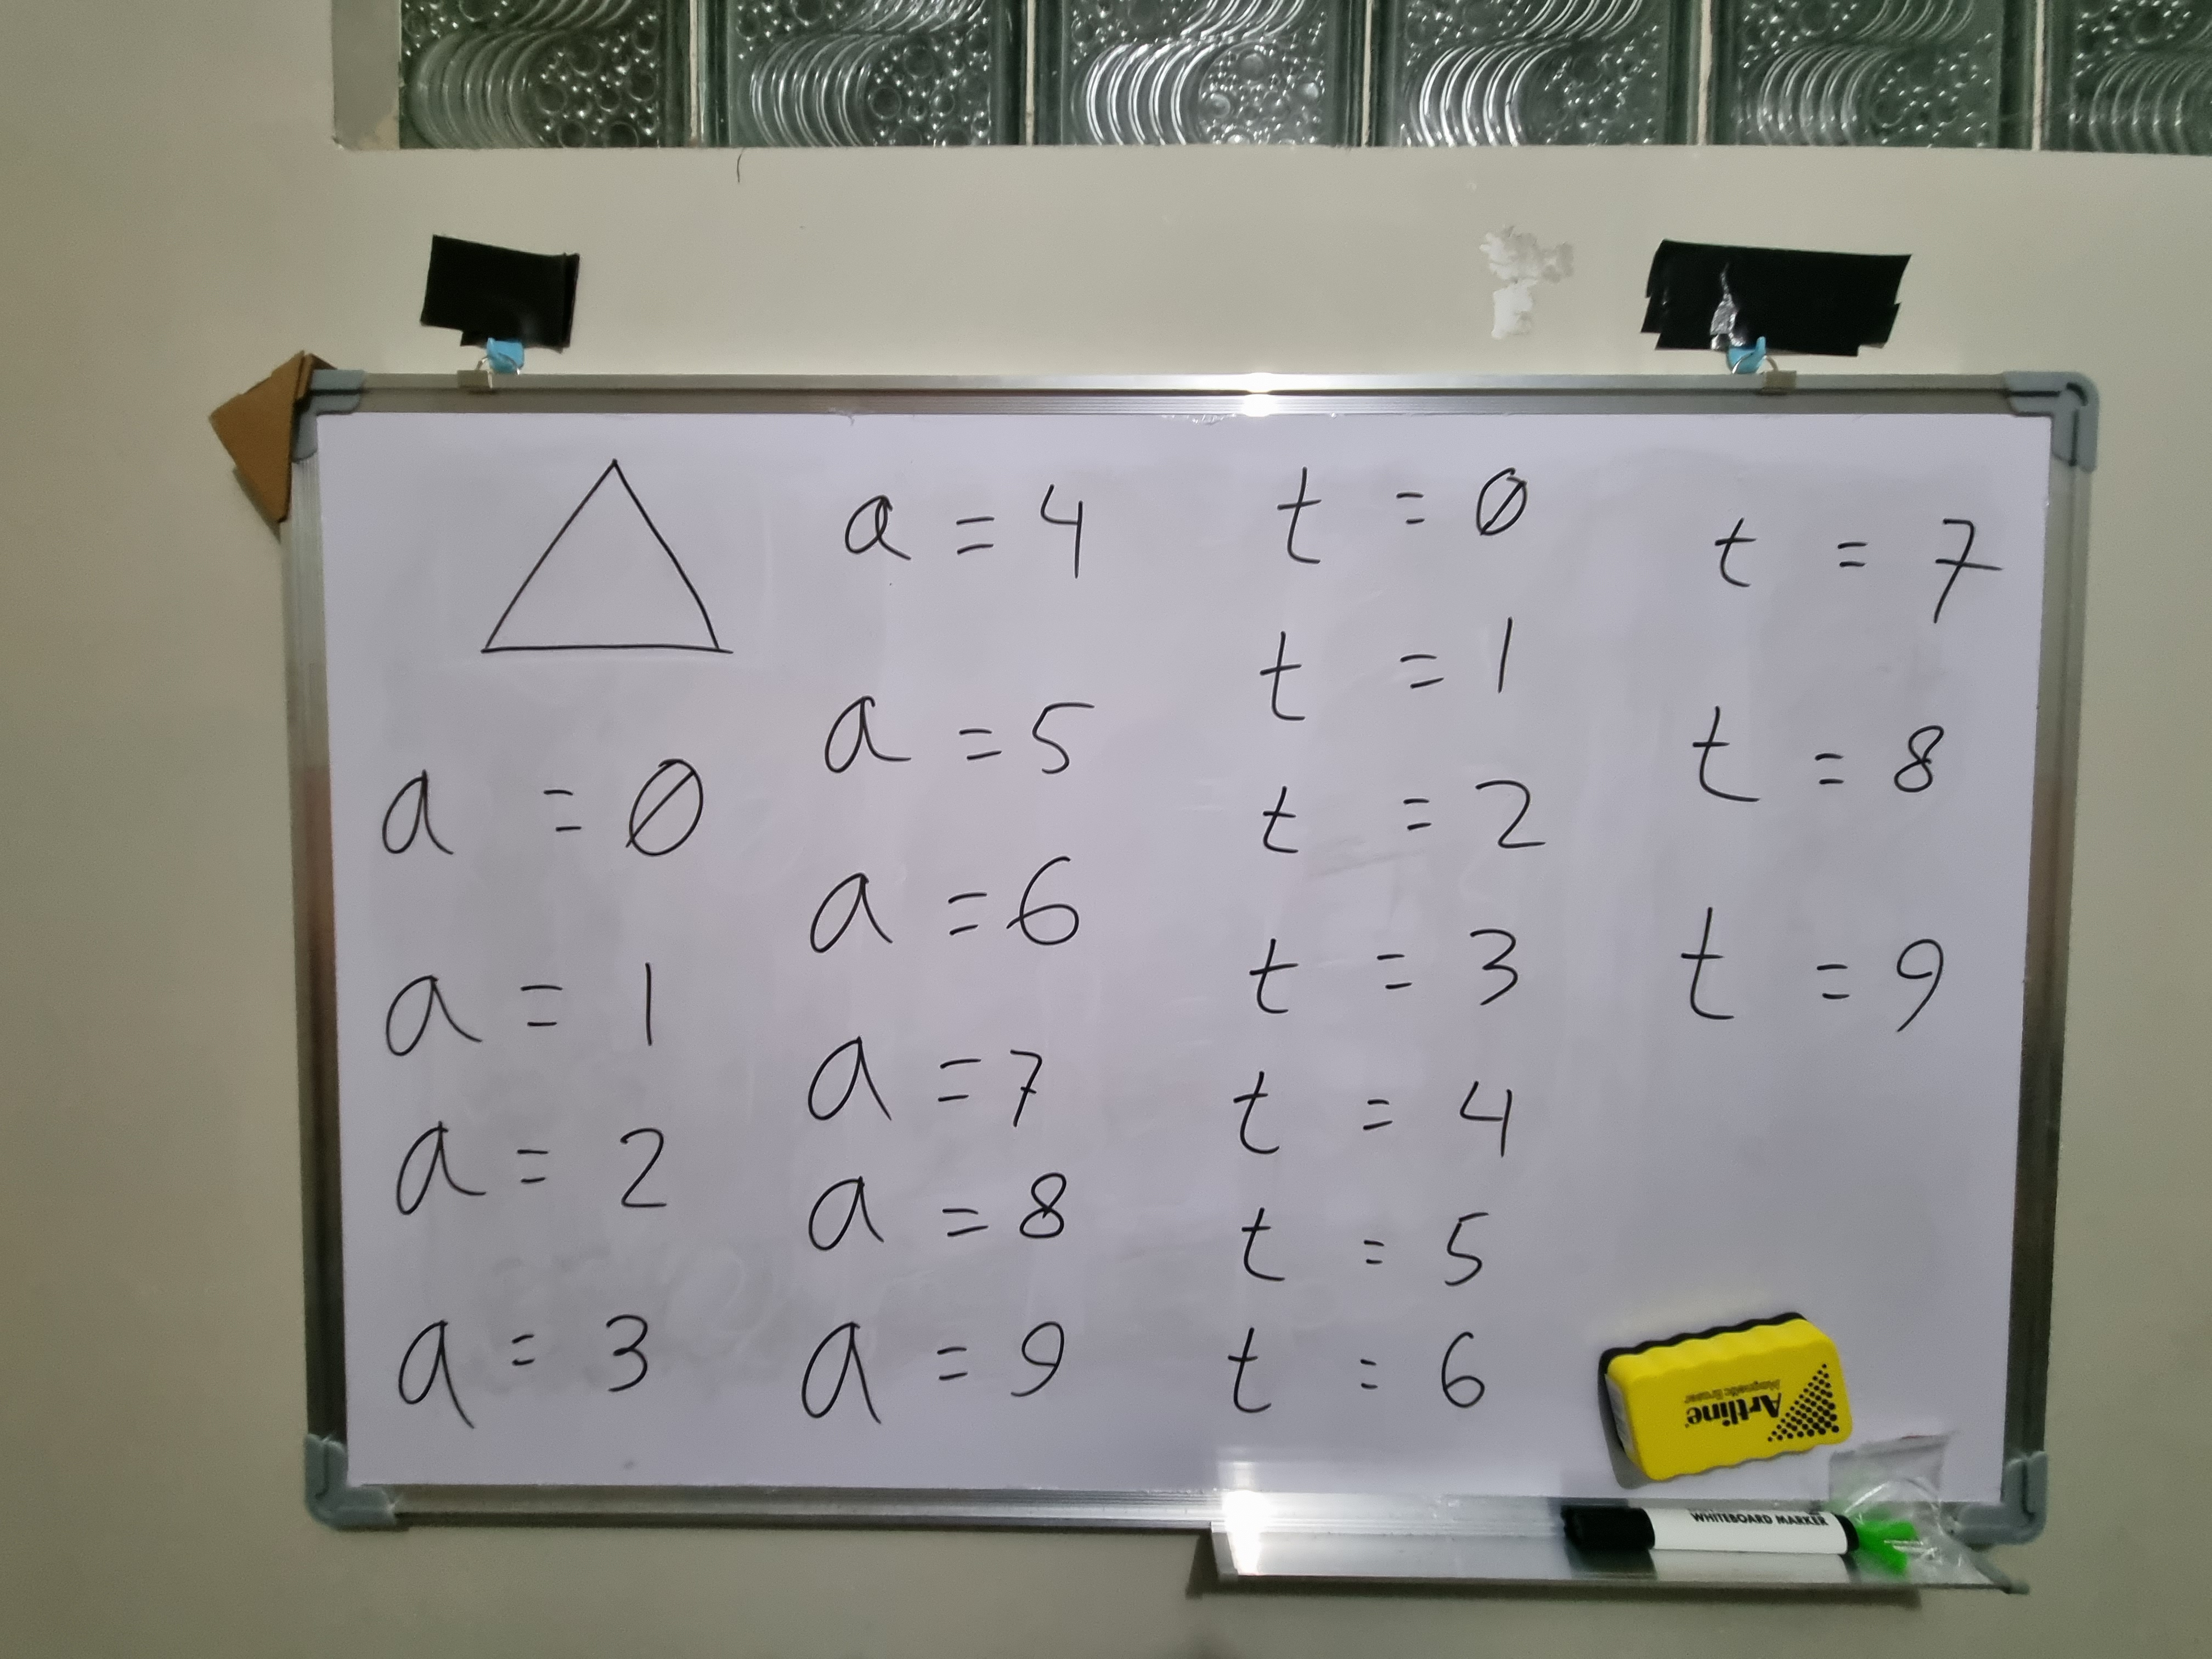
\includegraphics[width=0.55\textwidth]{gambar/Segitiga Dataset.jpg}	
	\captionof{figure}{Contoh Citra Gambar dan Parameter Bangun Segitiga}
	\label{fig:segitigaDataset}
\end{center}
Pada Gambar \ref{fig:segitigaDataset} didapatkan gambar bangun datar segitiga yang merupakan objek bangun datar yang akan dideteksi oleh program. Selain itu huruf "a" dan huruf "t" merupakan parameter yang akan dideteksi oleh program untuk mengetahui paramter dari sebuah bangun datar persegi. Angka "0" sampai "9" merupakan objek angka yang digunakan untuk perhitungan luas segitiga.

\begin{center}
	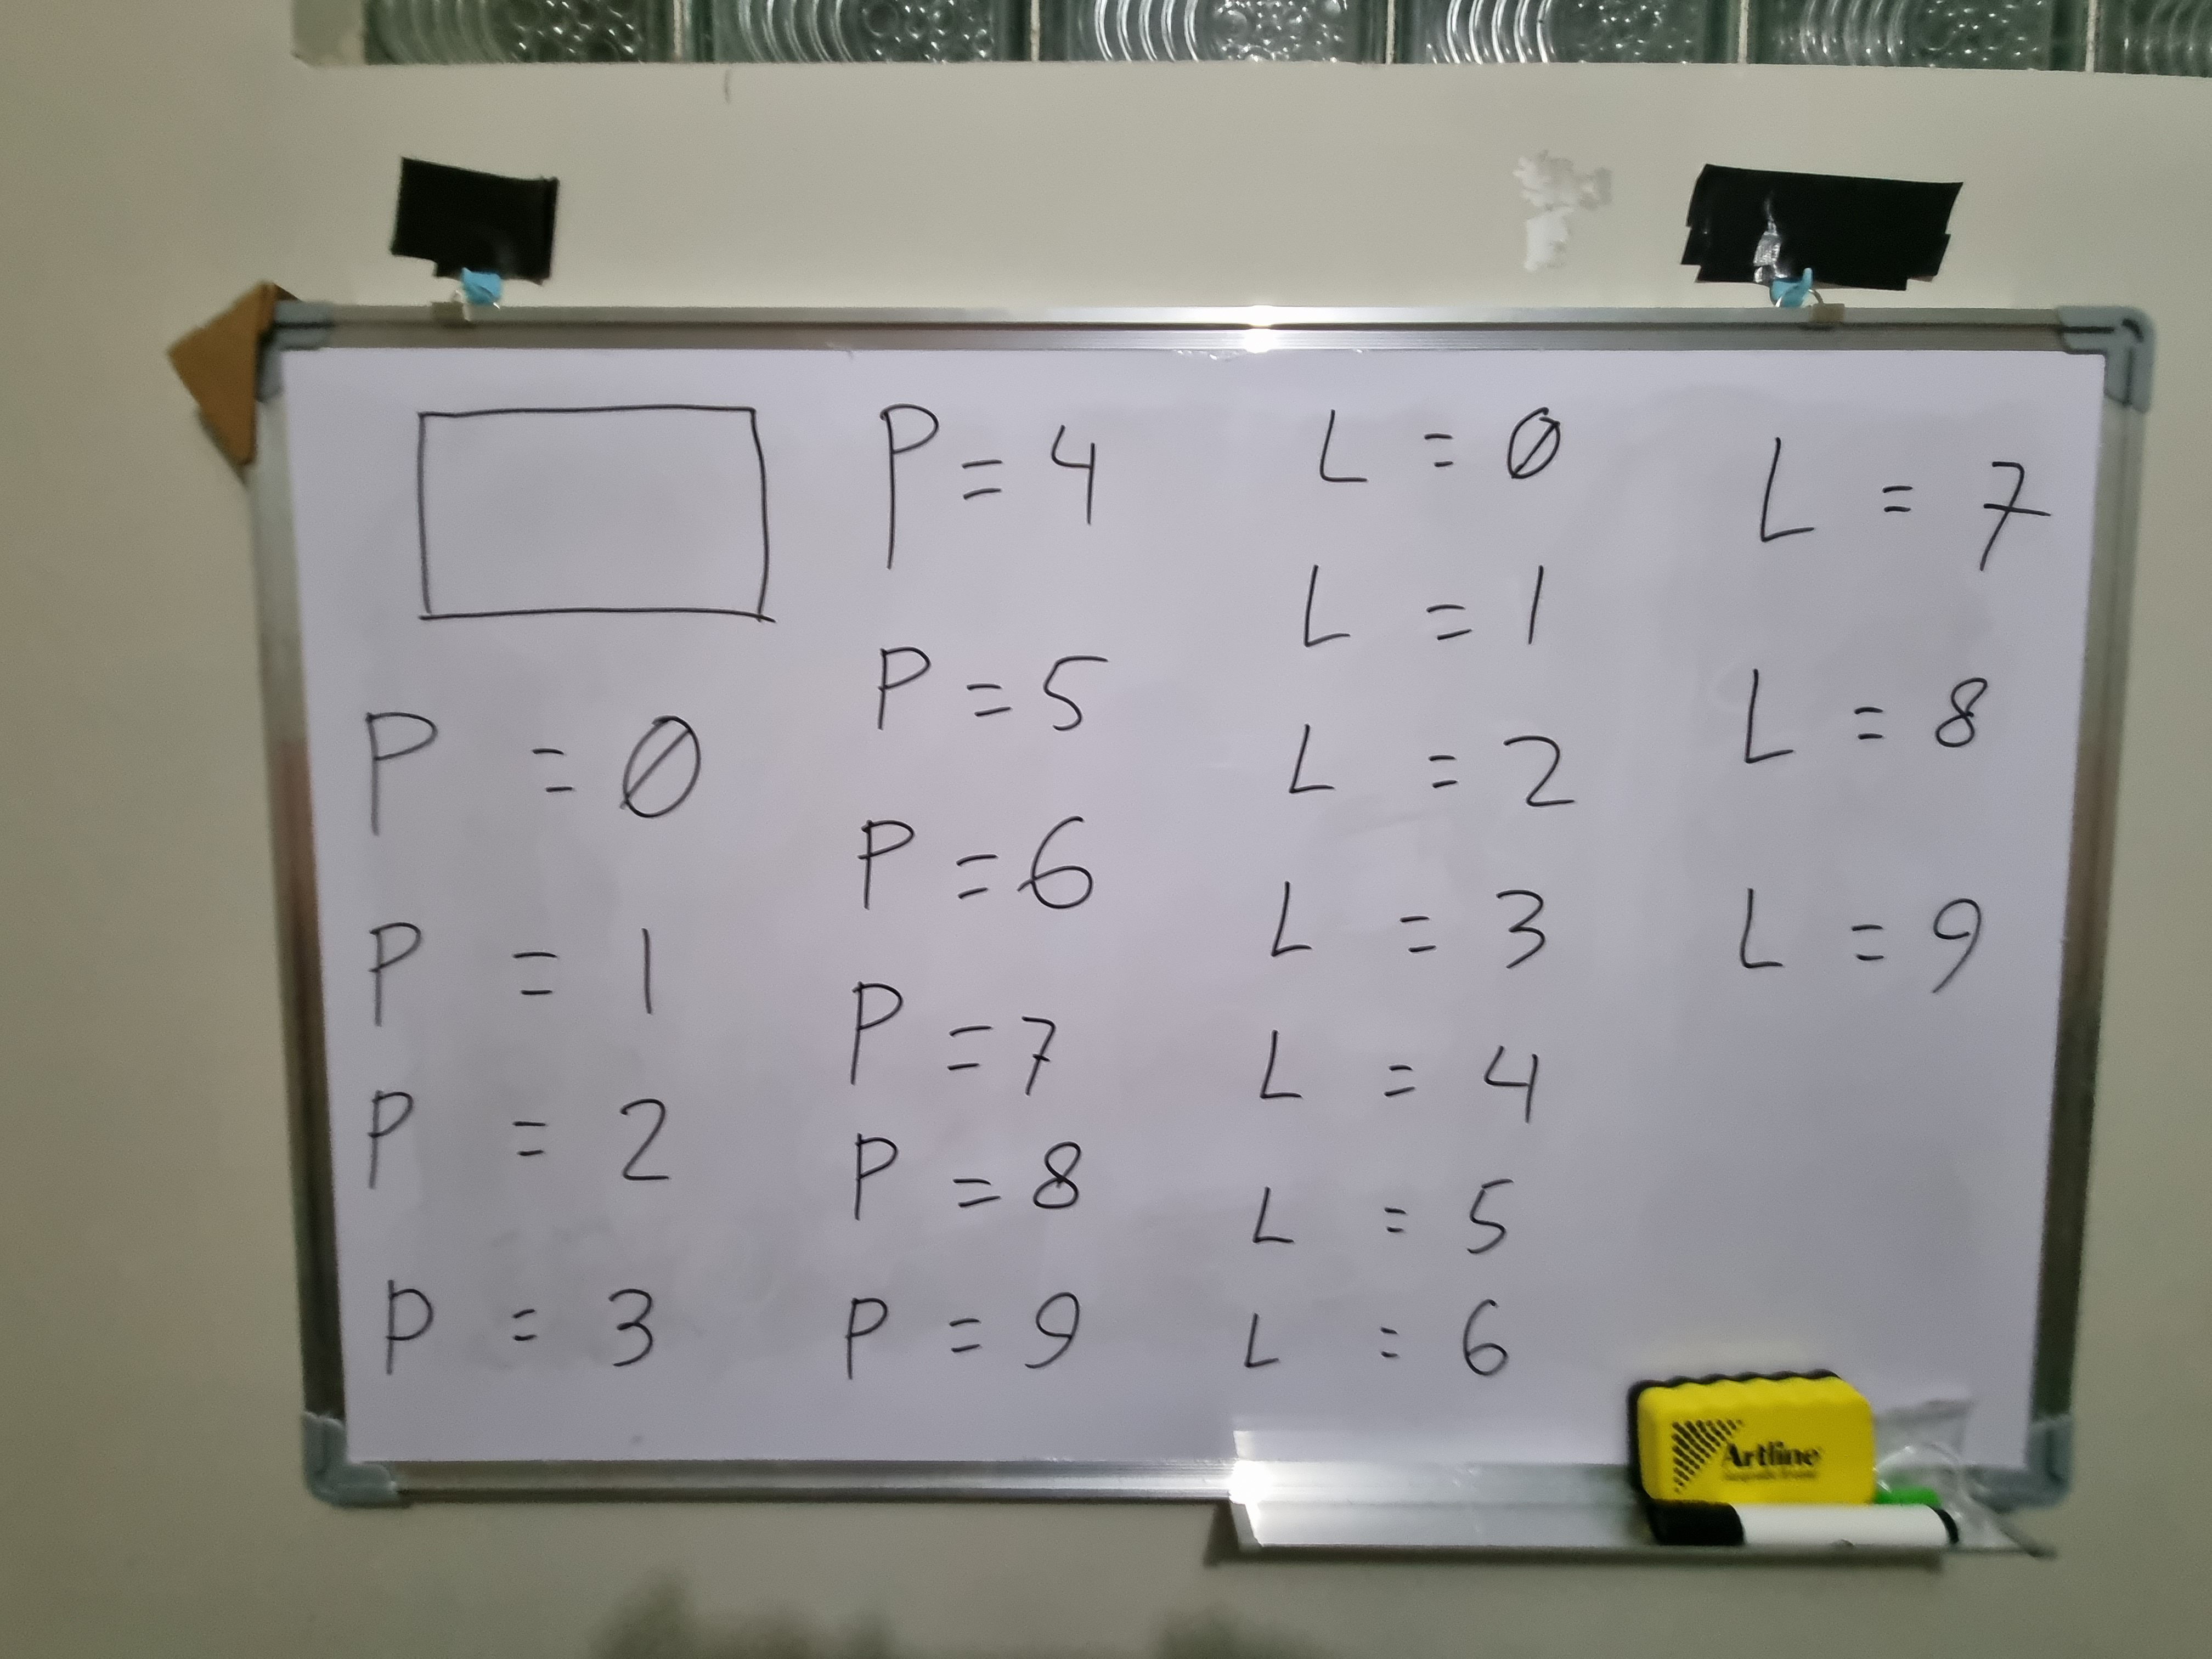
\includegraphics[width=0.55\textwidth]{gambar/Persegi Panjang Dataset.jpg}	
	\captionof{figure}{Contoh Citra Gambar dan Parameter Bangun Persegi Panjang}
	\label{fig:persegipanjangDataset}
\end{center}
Pada Gambar \ref{fig:persegipanjangDataset} didapatkan gambar bangun datar persegi panjang yang merupakan objek bangun datar yang akan dideteksi oleh program. Selain itu huruf "P" dan huruf "L" merupakan parameter yang akan dideteksi oleh program untuk mengetahui paramter dari sebuah bangun datar persegi. Angka "0" sampai "9" merupakan objek angka yang digunakan untuk perhitungan luas persegi panjang.

\begin{center}
	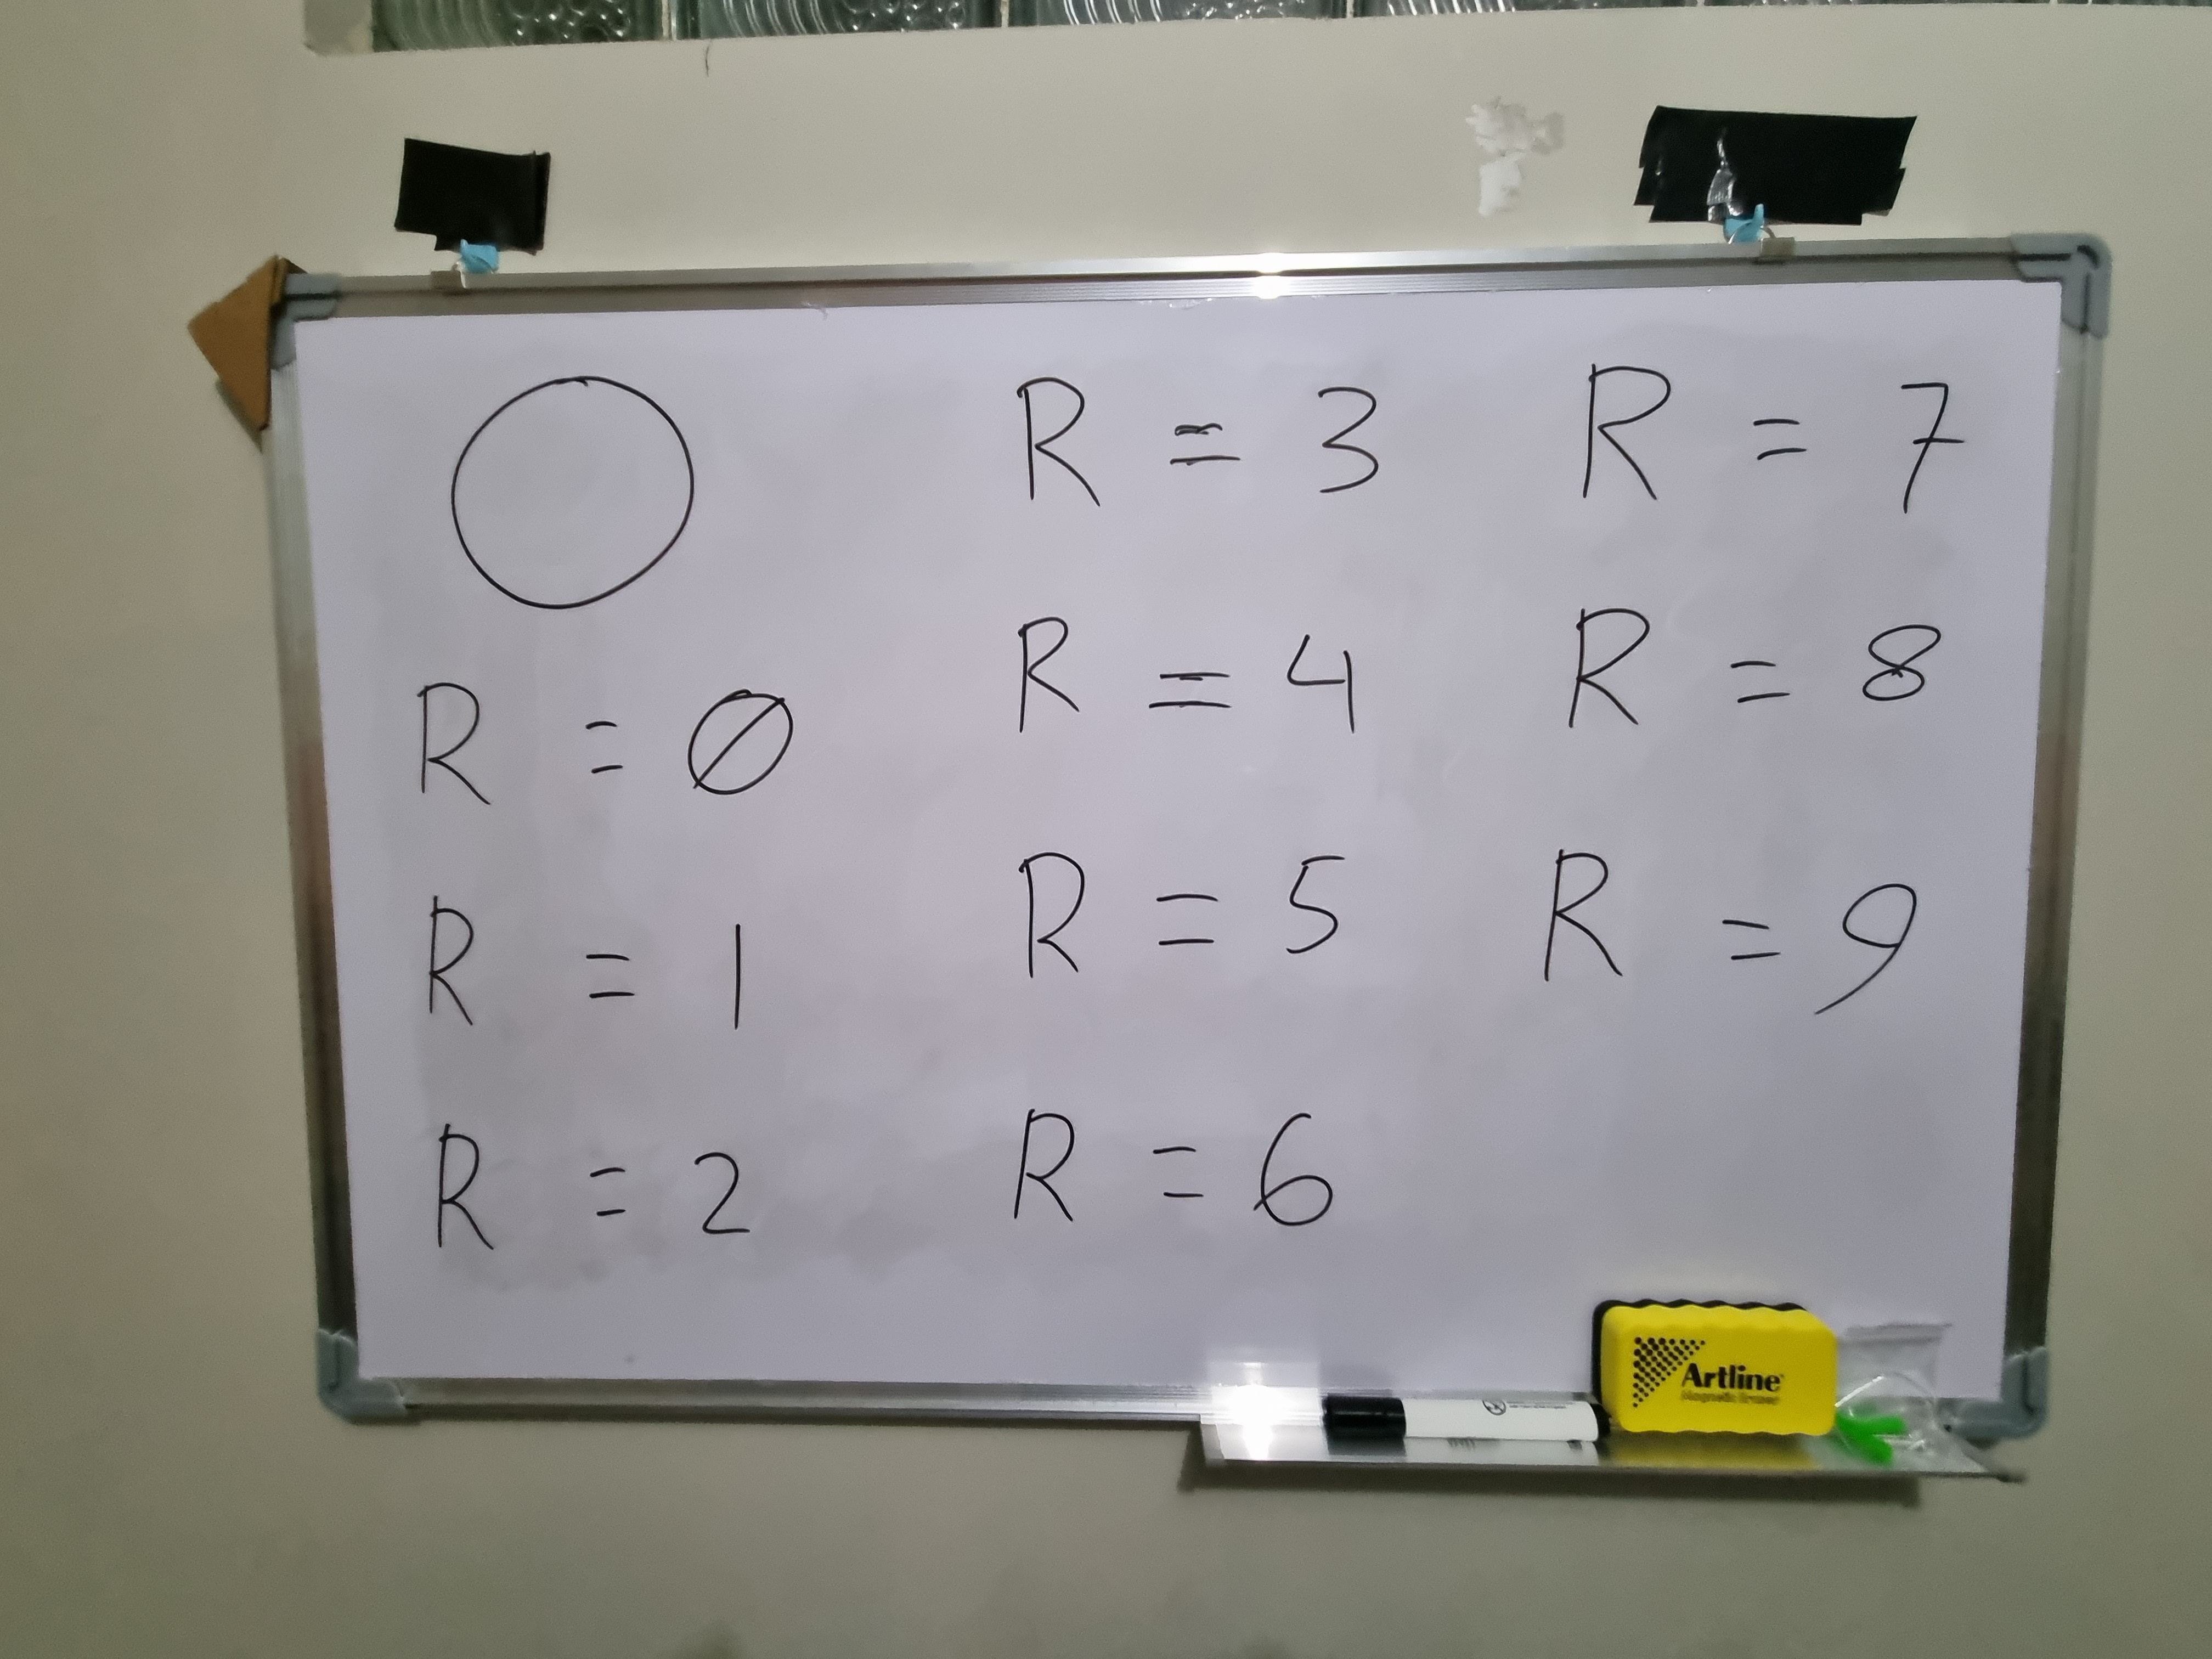
\includegraphics[width=0.55\textwidth]{gambar/Lingkaran Dataset.jpg}	
	\captionof{figure}{Contoh Citra Gambar dan Parameter Bangun Lingkaran}
	\label{fig:lingkaranDataset}
\end{center}
Pada Gambar \ref{fig:lingkaranDataset} didapatkan gambar bangun datar lingkaran yang merupakan objek bangun datar yang akan dideteksi oleh program. Selain itu huruf "R" merupakan parameter yang akan dideteksi oleh program untuk mengetahui paramter dari sebuah bangun datar persegi. Angka "0" sampai "9" merupakan objek angka yang digunakan untuk perhitungan luas lingkaran.

\begin{center}
	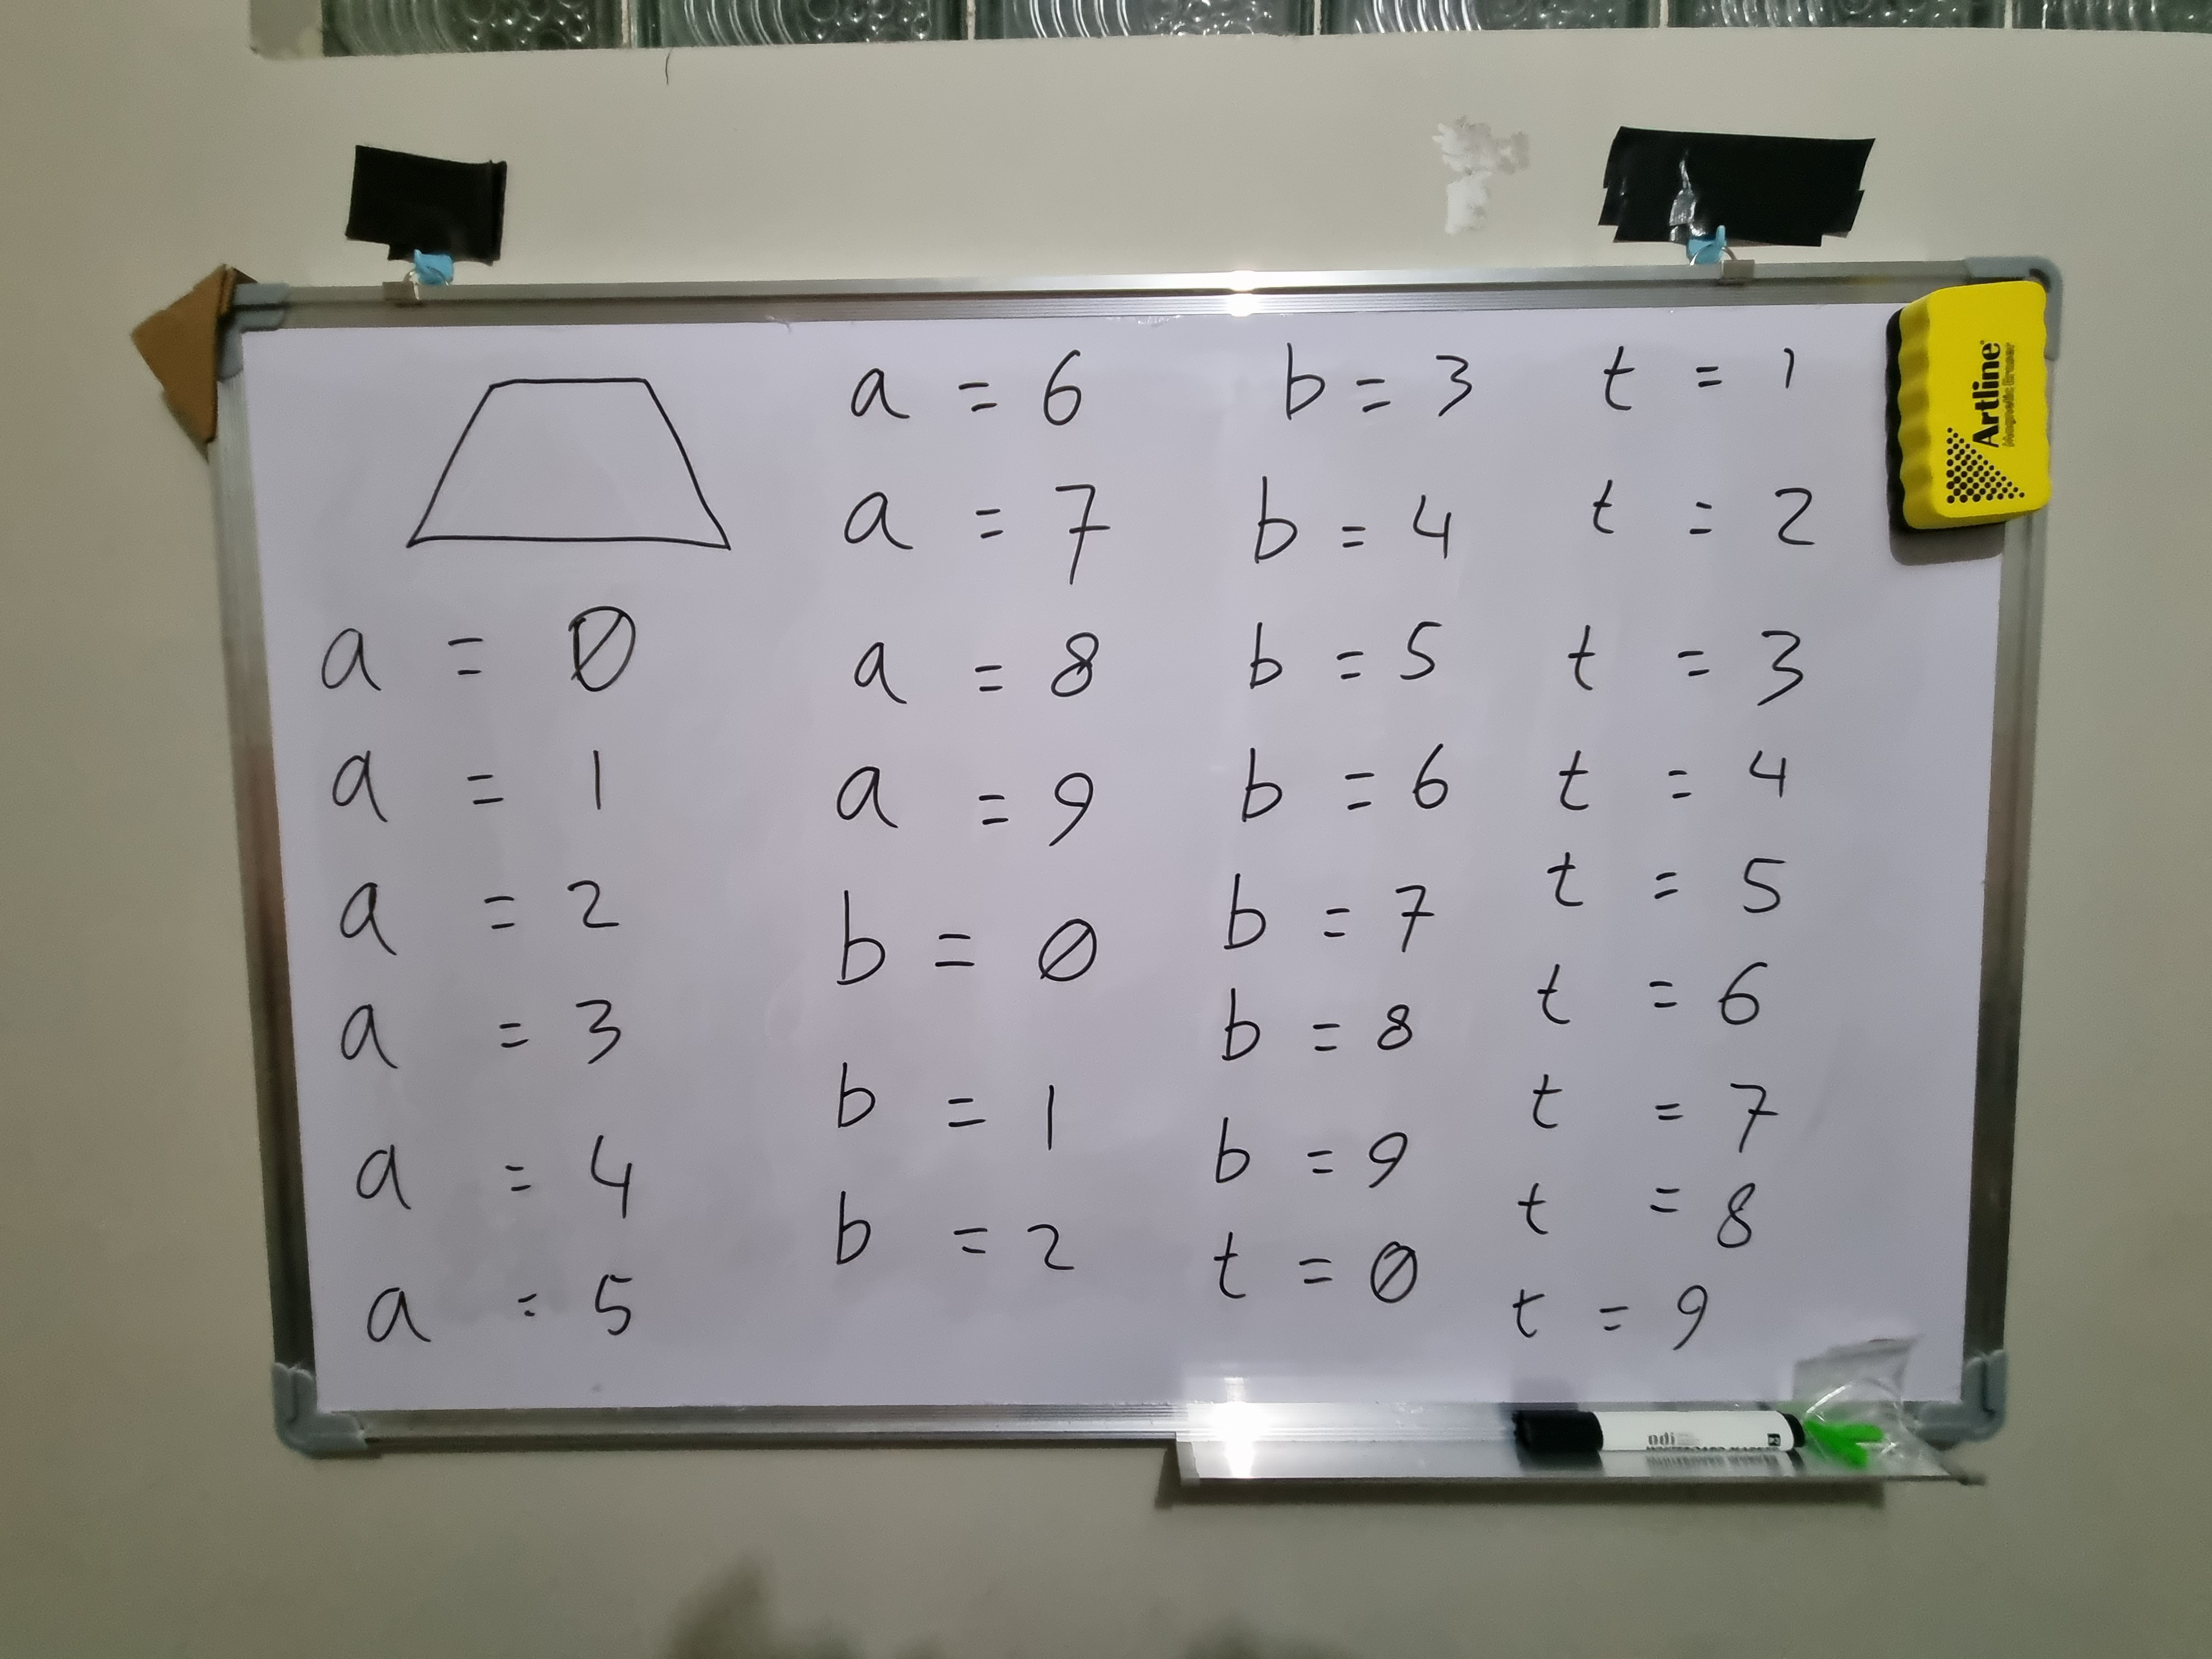
\includegraphics[width=0.55\textwidth]{gambar/Trapesium Dataset.jpg}
	\captionof{figure}{Contoh Citra Gambar dan Parameter Bangun Trapesium}
	\label{fig:trapesiumDataset}
\end{center}
Pada Gambar \ref{fig:trapesiumDataset} didapatkan gambar bangun datar trapesium yang merupakan objek bangun datar yang akan dideteksi oleh program. Selain itu huruf "a", huruf "b", dan huruf "t" merupakan parameter yang akan dideteksi oleh program untuk mengetahui paramter dari sebuah bangun datar persegi. Angka "0" sampai "9" merupakan objek angka yang digunakan untuk perhitungan luas trapesium.


\subsection{Pelabelan}
\label{subsubsec: hasil label dataset}
Proses pelabelan dilakukan dengan memberikan bounding box pada tiap citra yang telah dikumpulkan pada tahap \ref{subsection:Dataset}, alat bantu pelabelan yang digunakan adalah roboflow.
\begin{center}
	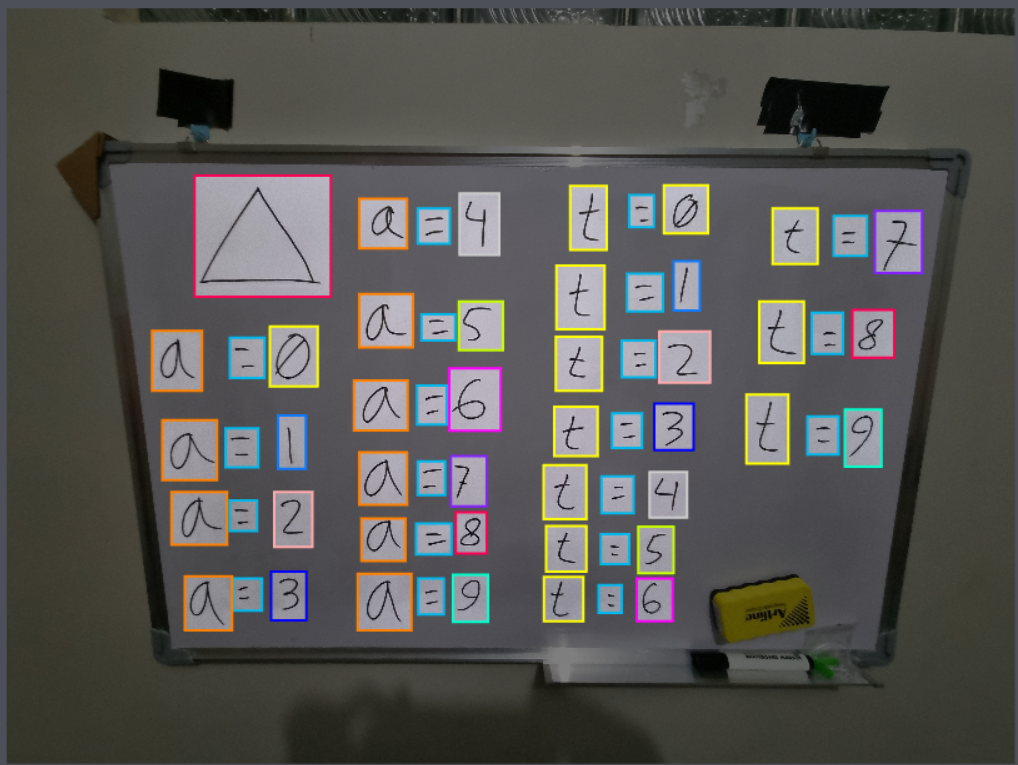
\includegraphics[width=0.55\textwidth]{gambar/labeling.png}
	\captionof{figure}{Proses pelabelan Bangun Datar Segitiga Menggunakan Roboflow}
	\label{fig:labelsegitiga}
\end{center}
Pelabelan pada Gambar \ref{fig:labelsegitiga} didapatkan gambar bangun datar segitiga yang merupakan objek bangun datar yang akan dideteksi oleh program. Selain itu huruf "a" dan huruf "t" merupakan parameter yang akan dideteksi oleh program untuk mengetahui paramter dari sebuah bangun datar persegi. Angka "0" sampai "9" merupakan objek angka yang digunakan untuk perhitungan luas segitiga.

\begin{center}
	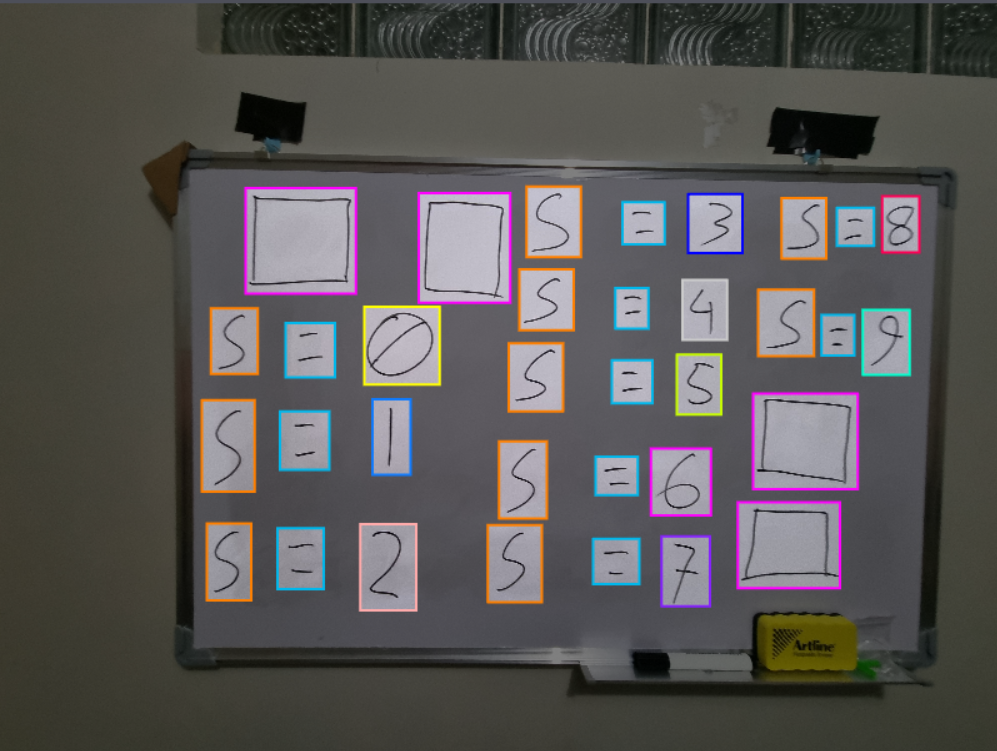
\includegraphics[width=0.55\textwidth]{gambar/Persegi Label.png}	
	\captionof{figure}{Proses pelabelan Bangun Datar Persegi Menggunakan Roboflow}
	\label{fig:persegiLabel}
\end{center}
Pelabelan pada Gambar \ref{fig:persegiLabel} didapatkan gambar bangun datar persegi yang merupakan objek bangun datar yang akan dideteksi oleh program. Selain itu huruf "S" merupakan parameter yang akan dideteksi oleh program untuk mengetahui paramter dari sebuah bangun datar persegi. Angka "0" sampai "9" merupakan objek angka yang digunakan untuk perhitungan luas persegi.

\begin{center}
	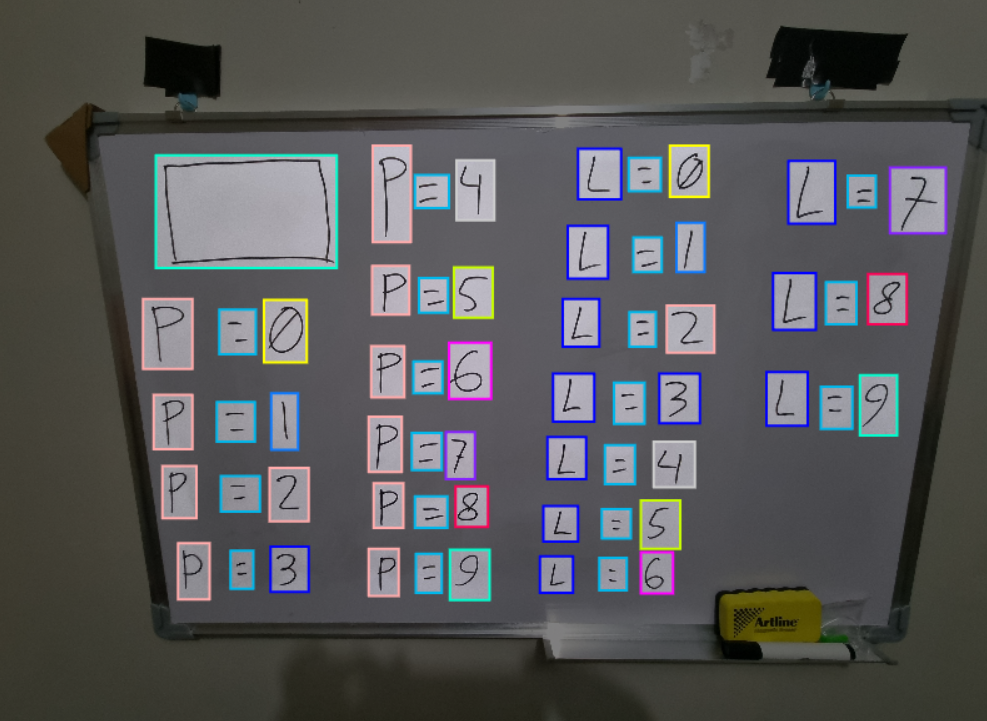
\includegraphics[width=0.55\textwidth]{gambar/Persegi Panjang Label.png}	
	\captionof{figure}{Proses pelabelan Bangun Datar Persegi Panjang Menggunakan Roboflow}
	\label{fig:persegipanjangLabel}
\end{center}
Pelabelan pada Gambar \ref{fig:persegipanjangLabel} didapatkan gambar bangun datar persegi panjang yang merupakan objek bangun datar yang akan dideteksi oleh program. Selain itu huruf "P" dan huruf "L" merupakan parameter yang akan dideteksi oleh program untuk mengetahui paramter dari sebuah bangun datar persegi. Angka "0" sampai "9" merupakan objek angka yang digunakan untuk perhitungan luas persegi panjang.

\begin{center}
	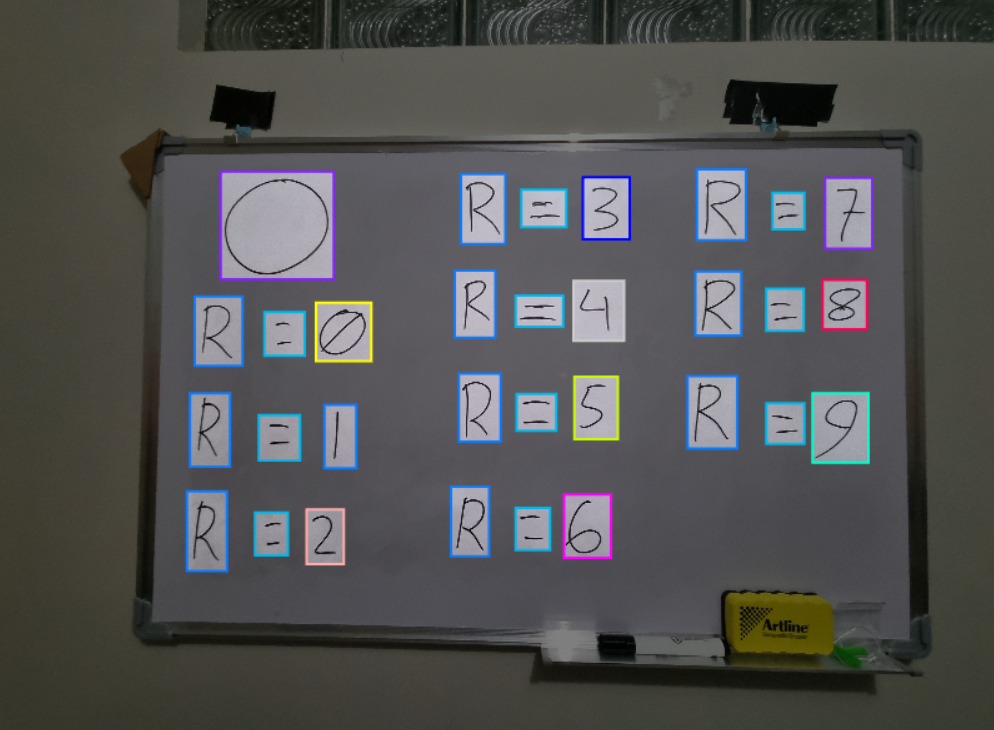
\includegraphics[width=0.55\textwidth]{gambar/Lingkaran Label.png}	
	\captionof{figure}{Proses pelabelan Bangun Datar Lingkaran Menggunakan Roboflow}
	\label{fig:lingkaranLabel}
\end{center}
Pelabelan pada Gambar \ref{fig:lingkaranLabel} didapatkan gambar bangun datar lingkaran yang merupakan objek bangun datar yang akan dideteksi oleh program. Selain itu huruf "R" merupakan parameter yang akan dideteksi oleh program untuk mengetahui paramter dari sebuah bangun datar persegi. Angka "0" sampai "9" merupakan objek angka yang digunakan untuk perhitungan luas lingkaran.

\begin{center}
	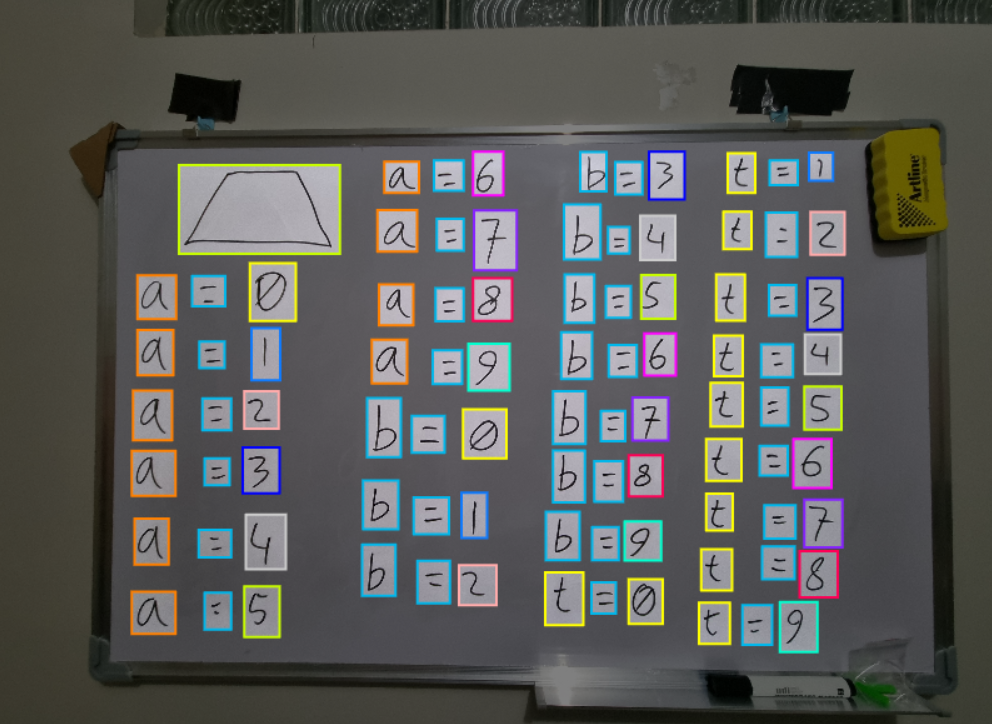
\includegraphics[width=0.55\textwidth]{gambar/Trapesium Label.png}
	\captionof{figure}{Proses pelabelan Bangun Datar Trapesium Menggunakan Roboflow}
	\label{fig:trapesiumLabel}
\end{center}
Pada Gambar \ref{fig:trapesiumLabel} didapatkan gambar bangun datar trapesium yang merupakan objek bangun datar yang akan dideteksi oleh program. Selain itu huruf "a", huruf "b", dan huruf "t" merupakan parameter yang akan dideteksi oleh program untuk mengetahui paramter dari sebuah bangun datar persegi. Angka "0" sampai "9" merupakan objek angka yang digunakan untuk perhitungan luas trapesium.

\subsection{Preprocessing Dataset}
\label{subsec:preproses}
Setelah dilakukan proses pelabelan pada tahap \ref{subsubsec: hasil label dataset}, output yang dihasilkan yaitu gambar yang memiliki \textit{bounding box}, dan apabila di-\textit{export} maka dataset hasil pelabelan terdiri dari 2 file yaitu file citra itu sendiri dan juga file txt yang berisi koordinat \textit{bounding box} yang ada pada suatu citra tersebut. Adapun total persebaran anotasi \textit{bounding box} pada masing-masing kelas dapat dilihat pada tabel \ref{tab:prep}.
\begin{table}[H]
\centering
	\caption{Anotasi bounding box untuk setiap kelas}
	\begin{tabular}{c c} 
		\toprule
		Kelas & Jumlah Anotasi \\ [0.5ex] 
		\midrule
		= & 2161 \\ 
		\midrule
		Lingkaran & 851 \\
		\midrule
		t & 647\\
		\midrule
		r & 630\\
		\midrule
		a & 605\\
		\midrule
		s & 522\\
		\midrule
		Segitiga & 495\\
		\midrule
		p & 404\\
		\midrule
		Persegi & 378\\
		\midrule
		Persegi Panjang & 371\\
		\midrule
		Trapesium & 371\\
		\midrule
		l & 376\\
		\midrule
		b & 337\\
		\midrule
		0 & 261\\
		\midrule
		1 & 299\\
		\midrule
		2 & 299\\
		\midrule
		3 & 299\\
		\midrule
		4 & 299\\
		\midrule
		5 & 299\\
		\midrule
		6 & 299\\
		\midrule
		7 & 299\\
		\midrule
		8 & 299\\
		\midrule
		9 & 296 \\ [1ex] 
		\bottomrule
	\end{tabular}
	\label{tab:prep}
\end{table}

Pada tahap \textit{pre-process}, citra yang telah diberi label selanjutnya diberikan sejumlah
proses \textit{bounding box rotation} agar didapatkan \textit{augmentasi} data untuk data \textit{training} dan memperbanyak jumlah dataset, selain itu dilakukan \textit{resize} sebesar gambar menjadi ukuran $416 \times 416$ sesuai dengan konfigurasi pada tabel \ref{tab:konfigyolo}, sehingga hasilnya seperti pada gambar \ref{fig:boxrot}.
\begin{center}
	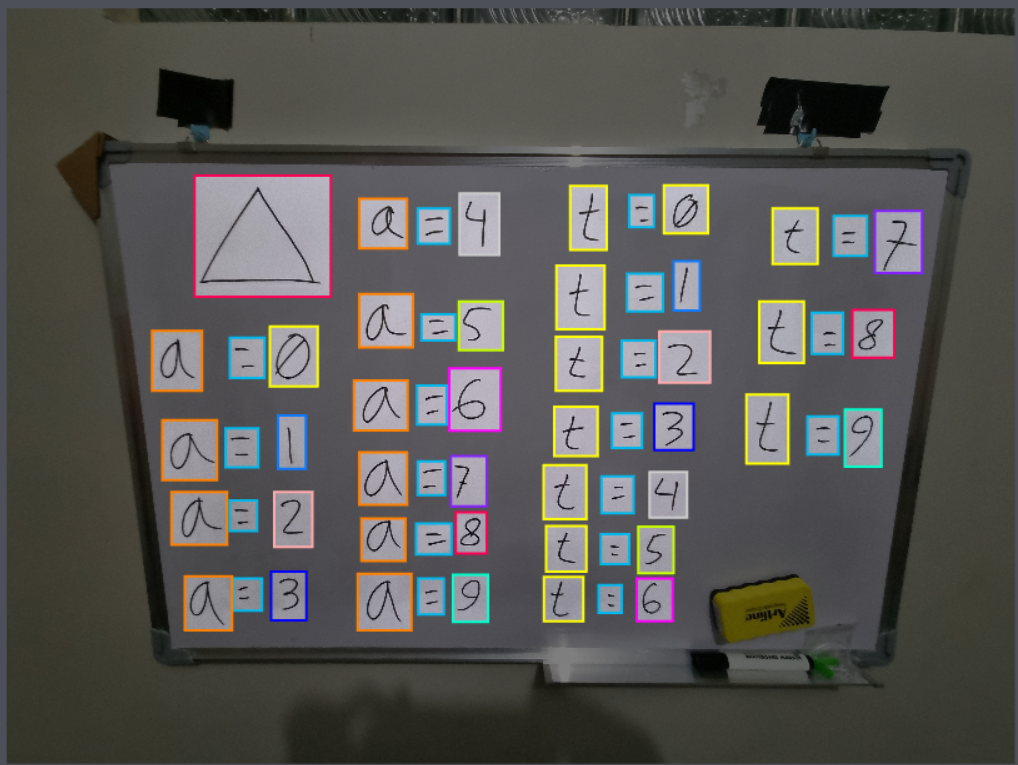
\includegraphics[width=0.55\textwidth]{gambar/labeling.png}
	\captionof{figure}{Sebelum rotasi bounding box}
	\label{fig:sebelumboxrot}
\end{center}
Pada Gambar \ref{fig:sebelumboxrot} didapatkan citra bangun datar dan parameternya yang telah diberikan label, selanjutnya akan diberikan \textit{augmentasi} \textit{bounding box rotation} dan \textit{resize} yang akan menghasilkan gambar seperti Gambar \ref{fig:boxrot}

\begin{center}
	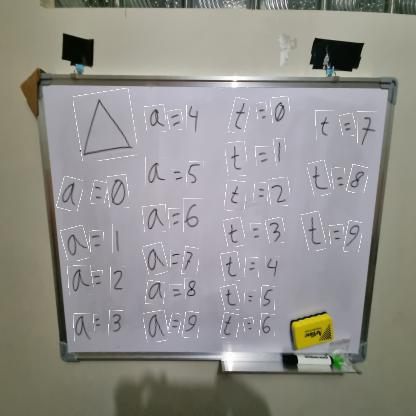
\includegraphics[width=0.55\textwidth]{gambar/boxrot.jpg}   
	\captionof{figure}{Gambar Sebelum dan Setelah Proses Bounding Box Rotation}
	\label{fig:boxrot}
\end{center}
Pada Gambar \ref{fig:boxrot} didapatkan citra bangun datar yang telah diberikan \textit{augmentasi} \textit{bounding box rotation} dan \textit{resize}, yang selanjutnya siap digunakan untuk proses \textit{training} yang akan dijelaskan pada tahap \ref{subsec: Training}.

\subsection{Training}
\label{subsec: Training}
Setelah didapatkan anotasi dari kelas-kelas objek yang dideteksi yang dilakukan pada tahap \ref{subsec:preproses}, hasil anotasi tersebut diteruskan menuju proses training. Proses ini bertujuan untuk melatih komputer dengan cara mengolah gambar dan anotasi yang telah dibuat sehingga terbentuk pola atau karakteristik dari masing-masing kelas yang akan menjadi bahan pertimbangan komputer dalam mencapai sebuah keputusan atau prediksi. 

Metode Yolov4-tiny digunakan dalam penelitian ini karena Yolov4-tiny dirancang berdasarkan metode Yolov4 untuk membuatnya memiliki kecepatan deteksi objek yang lebih cepat. Proses training menggunakan YOLOv4-tiny sebagai load weight dengan konfigurasi seperti Tabel \ref{tab:konfigyolo}. 
\begin{table}[H]
	\centering
	\caption{Konfigurasi YOLOv4-tiny}
	\begin{tabular}{|c|c|}
		\toprule
		Jenis Konfigurasi & Keterangan \\
		\midrule
		\textit{batch} & 64 \\  
		\midrule
		\textit{subdivision} & 32 \\
		\midrule
		\textit{width} & 416 \\
		\midrule
		\textit{height} & 416 \\
		\midrule
		\textit{Max\_batches} & 46000 \\
		\midrule
		\textit{Step} & 36800, 41400 \\
		\midrule
		\textit{classes} & 23 \\
		\midrule
		\textit{filters} & 84 \\
		\midrule
		\textit{scales} & .1,.1 \\
		\bottomrule
	\end{tabular}
	\label{tab:konfigyolo}\
\end{table}
Keterangan untuk setiap konfigurasi adalah sebagai berikut:
\begin{itemize}
	\item Jumlah \textit{batch} menentukan jumlah gambar yang akan diproses sebelum \textit{network weight} mengalami pembaharuan.
	\item Jumlah \textit{subdivision} bertujuan untuk memproses sebagian
	kecil \textit{batch size} sekaligus pada GPU.
	\item \textit{Max batches} merupakan batas iterasi dalam melakukan training yang didapatkan dengan cara \ref{item:maxbatch}. Yang berarti ketika iterasi sudah mencapai 46000, maka secara otomatis proses training akan berhenti.
	\item Karena jaringan YOLO menurunkan sampel input sebesar 32, kita hanya perlu memastikan \textit{width} dan \textit{height} adalah kelipatan 32, dan pada penelitian ini \textit{width} dan \textit{height} yang digunakan adalah $416 \times 416$.
	\item Nilai \textit{steps} merupakan nilai \textit{checkpoint} (jumlah iterasi) di mana skala belajar akan diterapkan, pada penelitian ini nilai step yang digunakan adalah 36800 dengan skala belajar yang diterapkan adalah $0.1$ dan 41400 dengan skala belajar yang diterapkan adalah $0.1$.
	\item \textit{class} pada konfigurasi diatur menjadi 23 karena \textit{class} dataset saat diberikan pelabelan pada tahap \ref{subsubsec: hasil label dataset} memiliki 23 \textit{class}.
	\item Nilai \textit{filters} didapatkan dengan cara \ref{item:filter} karena Yolov4-tiny mendeteksi 3 kotak per sel grid fitur dan untuk setiap kotak akan memprediksi probabilitas $\textit{class} + \textit{width} + \textit{height} + x + y + \textit{confidence}$.
\end{itemize}
Nilai   Nilai max batches, steps, dan filters ditentukan dengan cara berikut:
\begin{itemize}
	\item $max\_batches = jumlahclass \times  2000$ \label{item:maxbatch}
	\item $steps = (80\%max batches), (90\%max batches)$
	\item $filters = (jumlahkelas + 5) \times 3$ \label{item:filter}
\end{itemize}
selanjutnya dilakukan tahap training yang akan menghasilkan bobot (weight) yang akan digunakan untuk tahap training. Pada penelitian ini terdapat sebuah perangkat laptop yang digunakan untuk melakuan testing pada model yang sudah jadi 
dan membuat prototype sistem untuk menerapkan model yang sudah jadi menggunakan input gambar dengan spesifikasi seperti yang terdapat pada Tabel \ref{tab:spesifikasilaptop}.
\begin{table}[H]
\centering
	\caption{Spesifikasi Laptop}
	\begin{tabular}{|c|c|}
		 \toprule
		 Merk Laptop & Asus ROG GL503VM \\
		 \midrule
		 Processor & Intel(R) Core(TM) i7-770HQ CPU @ 2.80GHz (8 CPUs), ~2.8GHz \\  
		 \midrule
		 Operating System & Windows 10  \\
		 \midrule
		 Graphics & Geforce GTX 1060 Laptop GPU 6GB DDR4 \\
		 \midrule
		 Webcam & 720p \\
		 \midrule
		 Memory & 6GB \\
		 \midrule
		 Storage & 1TB \\
		 \bottomrule
	\end{tabular}
	\label{tab:spesifikasilaptop}\
\end{table}

\subsection{Testing dan output}
Proses ini, diawali dengan melakukan pengujian pada model (weight) hasil \textit{training} yang telah didapatkan dengan menggunakan Testing dataset sehingga didapatkan nilai TP, FP, dan FN. Setelah itu, pengujian juga dilakukan dengan meng-\textit{input}-kan gambar atau video baik video hasil rekaman maupun real-time video. Kemudian dilakukan deteksi dan klasifikasi tulisan tangan huruf, angka, dan bangun datar pada gambar atau video yang telah di-\textit{input}-kan tersebut dengan menggunakan model yang telah didapatkan sebelumnya. Setelah itu, akan diperoleh dimensi dari objek yang dideteksi. Dengan ada dimensi objek yaitu tulisan tangan huruf, angka, dan operator aritmatika, maka output dari sistem akan memberikan \textit{bounding box} pada objek yang terdeteksi. Kemudian label juga akan diberikan pada \textit{bounding box} tersebut.

Lalu \textit{bounding box} akan diurutkan oleh program, yang mana apabila belum mencapai \textit{threshold} tertentu tidak akan membuat baris yang baru, namun apabila sudah melebihi \textit{threshold tertentu} akan membuat baris yang baru. setelah dilakukan pengurutan, selanjutnya adalah mengambil angka untuk dilakukan proses selanjutnya, yaitu perhitungan dengan rumus bangun datar yang terdeteksi. Rumus yang digunakan oleh program tergantung dari bangun yang terdeteksi pada awal pendeteksian. Apabila ada salah satu bangun datar, huruf, atau angka yang tidak terdeteksi, maka hasil yang dikeluarkan adalah teks "ada yang tidak terdeteksi", atau "..." apabila bangun datar tidak terdeteksi sama sekali.

%Deteksi dan klasifikasi parameter bangun datar pada papan tulis menggunakan tulisan tangan dilakukan setelah melakukan training pada YOLO, Gambar \ref{fig:segitigatest} sampai Gambar \ref{fig:persegipanjangtest} adalah hasil deteksi parameter bangun datar menggunakan beberapa sampel dari masing-masing lima bangun datar.
%\begin{center}
%	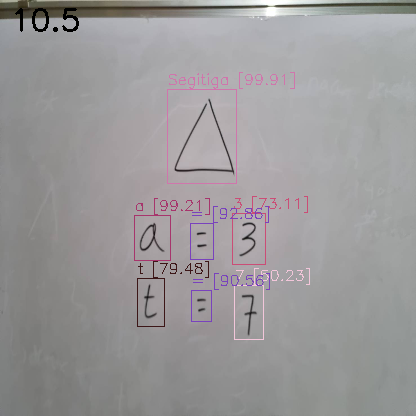
\includegraphics[width=0.75\textwidth]{gambar/segitiga2.png}
%	\captionof{figure}{Deteksi Segitiga dan Hasilnya}
%	\label{fig:segitigatest}
%\end{center}
%Pada Gambar \ref{fig:segitigatest} didapatkan berhasilnya deteksi daripada gambar bangun datar segitiga beserta parameter huruf dan angka, yang mengakibatkan berhasilnya perhitungan luas yang mana hasil dari perhitungan luas diletakkan pada pojok kiri atas \textit{window} gambar.
%
%\begin{center}
%	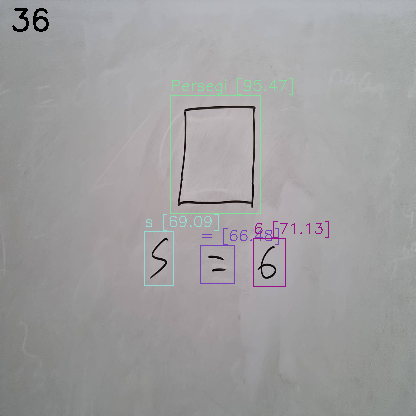
\includegraphics[width=0.75\textwidth]{gambar/persegi2.png}
%	\captionof{figure}{Deteksi Persegi dan Hasilnya}
%	\label{fig:persegitest}
%\end{center}
%Pada Gambar \ref{fig:persegitest} didapatkan berhasilnya deteksi daripada gambar bangun datar persegi beserta parameter huruf dan angka, yang mengakibatkan berhasilnya perhitungan luas yang mana hasil dari perhitungan luas diletakkan pada pojok kiri atas \textit{window} gambar.
%
%\begin{center}
%	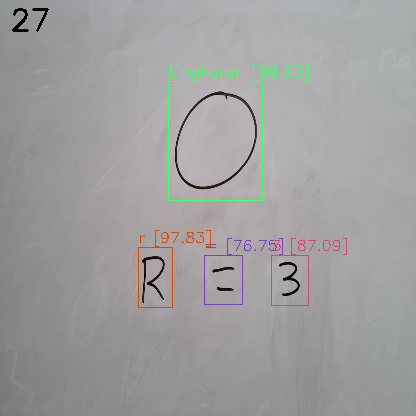
\includegraphics[width=0.75\textwidth]{gambar/lingkaran2.png}
%	\captionof{figure}{Deteksi Lingkaran dan Hasilnya}
%	\label{fig:lingkarantest}
%\end{center}
%Pada Gambar \ref{fig:lingkarantest} didapatkan berhasilnya deteksi daripada gambar bangun datar lingkaran beserta parameter huruf dan angka, yang mengakibatkan berhasilnya perhitungan luas yang mana hasil dari perhitungan luas diletakkan pada pojok kiri atas \textit{window} gambar.
%
%\begin{center}
%	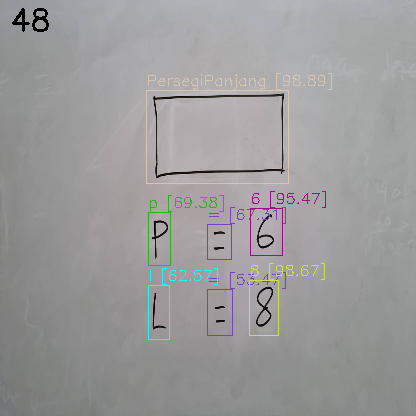
\includegraphics[width=0.75\textwidth]{gambar/persegi panjang2.png}
%	\captionof{figure}{Deteksi Persegi Panjang dan Hasilnya}
%	\label{fig:persegipanjangtest}
%\end{center}
%Pada Gambar \ref{fig:persegipanjangtest} didapatkan tidak sepenuhnya berhasil deteksi daripada gambar bangun datar persegi panjang beserta parameter huruf dan angka, yang mengakibatkan tidak berhasilnya perhitungan luas yang mana hasil dari gagalnya perhitungan luas diletakkan pada pojok kiri atas \textit{window} gambar dengan penjelasan "ada yang tidak terdeteksi".
%
%\begin{center}
%	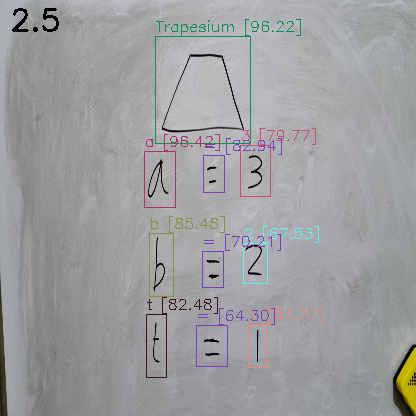
\includegraphics[width=0.75\textwidth]{gambar/trapesium2.png}
%	\captionof{figure}{Deteksi Trapesium dan Hasilnya}
%	\label{fig:trapesiumtest}
%\end{center}
%Pada Gambar \ref{fig:trapesiumtest} didapatkan tidak sepenuhnya berhasil deteksi daripada gambar bangun datar trapesium beserta parameter huruf dan angka, yang mengakibatkan tidak berhasilnya perhitungan luas yang mana hasil dari gagalnya perhitungan luas diletakkan pada pojok kiri atas \textit{window} gambar dengan penjelasan "ada yang tidak terdeteksi".